\chapter{Exercises with answers}

\begin{Exercise} [
  title={Coding sequence},
  difficulty={1},
  label={excs},
  origin={G. Valle}
 ]

 \begin{figure}[H]
  \centering
  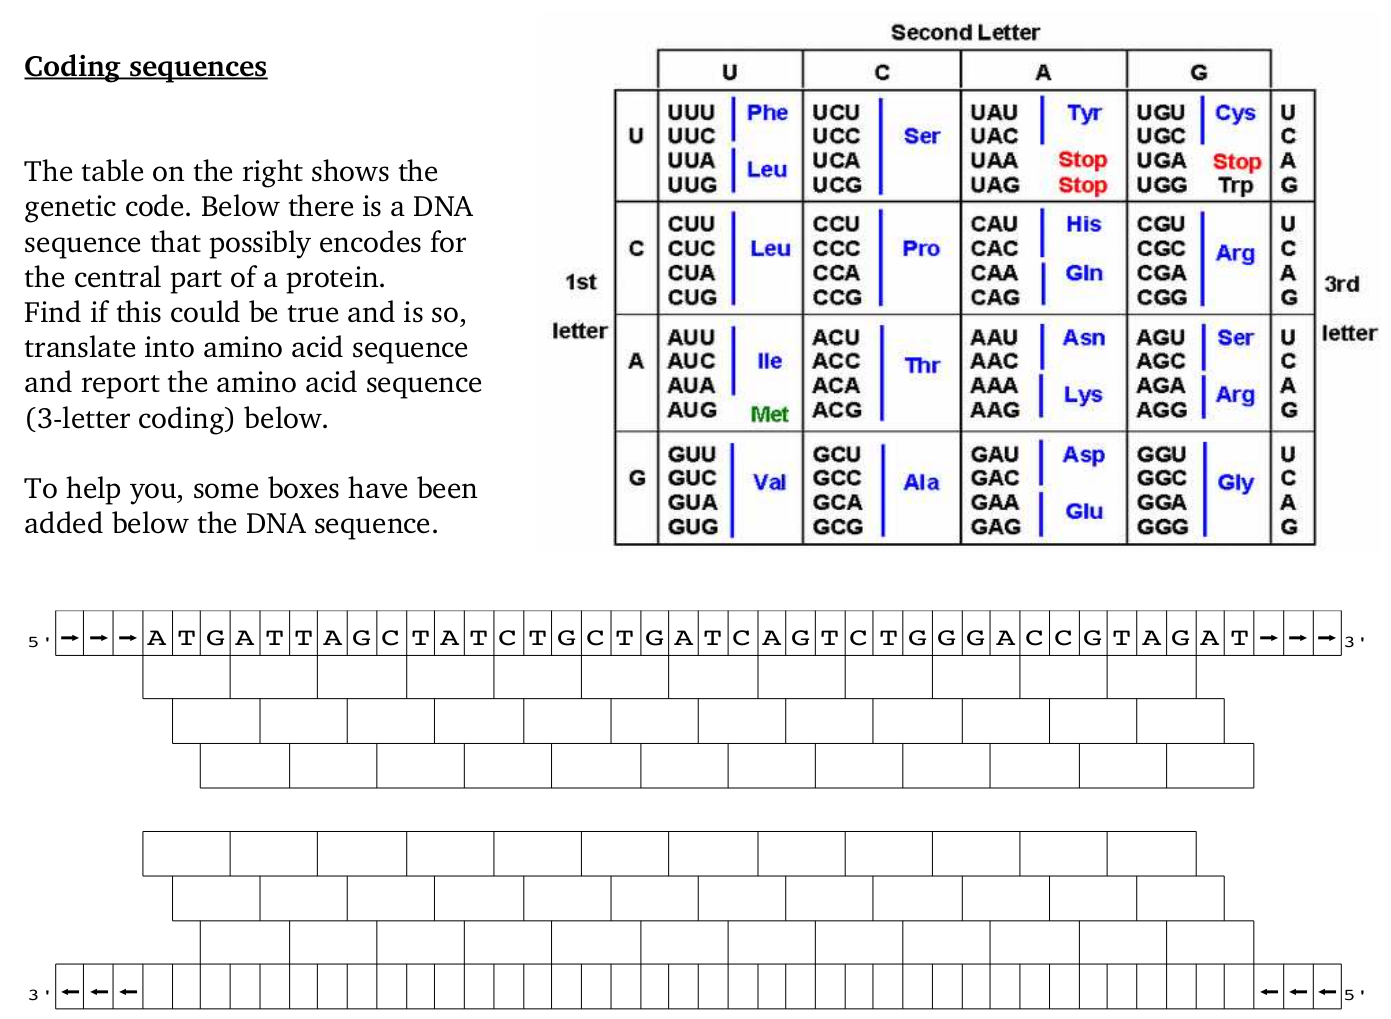
\includegraphics[scale=0.3]{Find_coding_sequence}
 \end{figure}

\end{Exercise}

\newpage

\begin{Answer} [
  ref={excs},
  number={1}
 ]

 \begin{figure}[H]
  \centering
  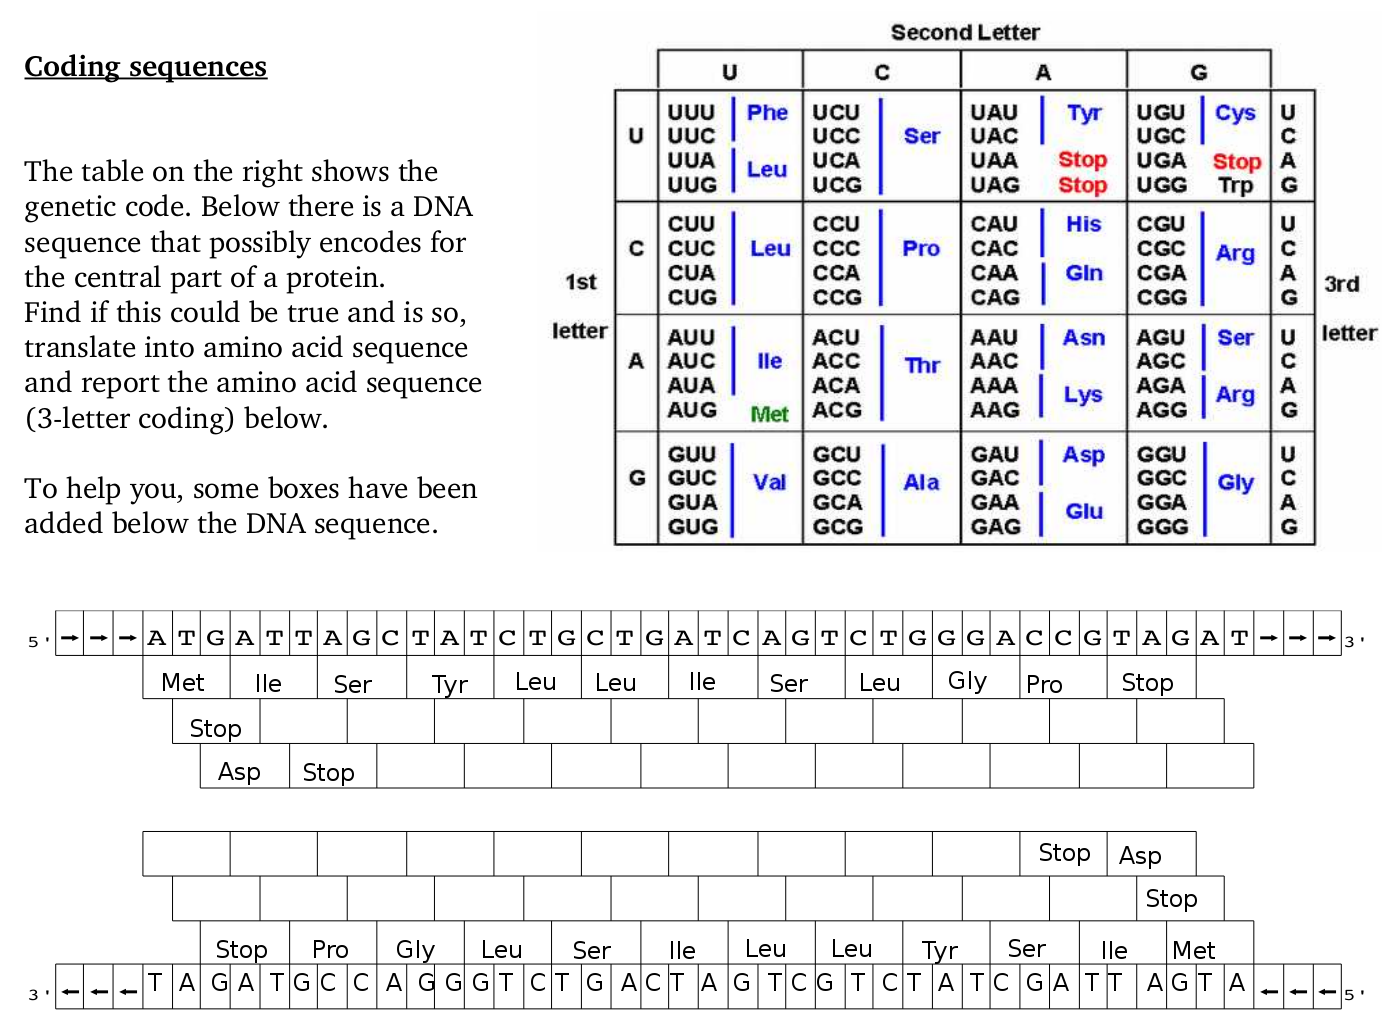
\includegraphics[scale=0.3]{Find_coding_sequence_sol}
 \end{figure}

\end{Answer}



\begin{Exercise} [
  title={Chromosomes},
  difficulty={1},
  label={ex1},
  origin={G. Valle}
 ]

  In adult human cells there are 46 chromosomes. De novo mutations are generally
very rare and we are not considering them in the following reasoning.
Answer \textbf{True} or \textbf{False}:

  \Question 23 chromosome are inherited from the mother and 23 from the father
  \Question Each chromosome of a child must have an identical copy in one of the
2 parents
  \subQuestion Explain why
\end{Exercise}

\begin{Answer} [
   ref={ex1},
   number={1}
 ]

  \Question \textbf{True}
  \Question \textbf{False}
  \subQuestion The second statement is wrong because of the crossing over

\end{Answer}


\begin{Exercise} [
  title={Genomes and genes},
  difficulty={1},
  label={ex2},
  origin={G. Valle}
 ]

  Approximately, how big is the genome and how many genes are there...

  \Question In a bacterium like \textbf{E. Coli}
  \Question In a simple eukaryote like \textbf{yeast}
  \Question In humans

\end{Exercise}

\begin{Answer} [
  ref={ex2},
  number={2}
 ]

  \Question Genome size: 100 Mbp. Number of genes: 19000 (27\% encoding)
  \Question Genome size: 13 Mbp. Number of genes: 6000 (70\% encoding)
  \Question Genome size: 3000 Mbp. Number of genes: 23000/25000 (1.5\% encoding)

\end{Answer}

\begin{Exercise} [
  title={Enzyme},
  difficulty={1},
  label={ex3},
  origin={G. Valle}
 ]

  Answer the questions.

  \Question How is called the enzyme that duplicate the DNA?
  \Question How is called the enzyme that transcribes DNA into RNA?
  \Question How is it called the biological structure where proteins are
synthesized?
\end{Exercise}

\begin{Answer} [
  ref={ex3},
  number={3}
 ]

  \Question DNA Polymerase
  \Question RNA Polymerase
  \Question Ribosome
\end{Answer}

\begin{Exercise} [
  title={Smith and Waterman algorithm},
  difficulty={1},
  label={exSW},
  origin={G. Valle}
 ]

 Consider the following two sequences:

 \begin{itemize}
  \item \texttt{DFTLNL}
  \item \texttt{EYSHMC}
 \end{itemize}

 Simulate the Smith-Waterman algorithm using the PAM240 and a gap penalty of
 4 points, both for starting and extending the gap.
 Finally, report the two aligned sequences below and the final score of the
 alignment.

 \begin{figure}[H]
  \centering
  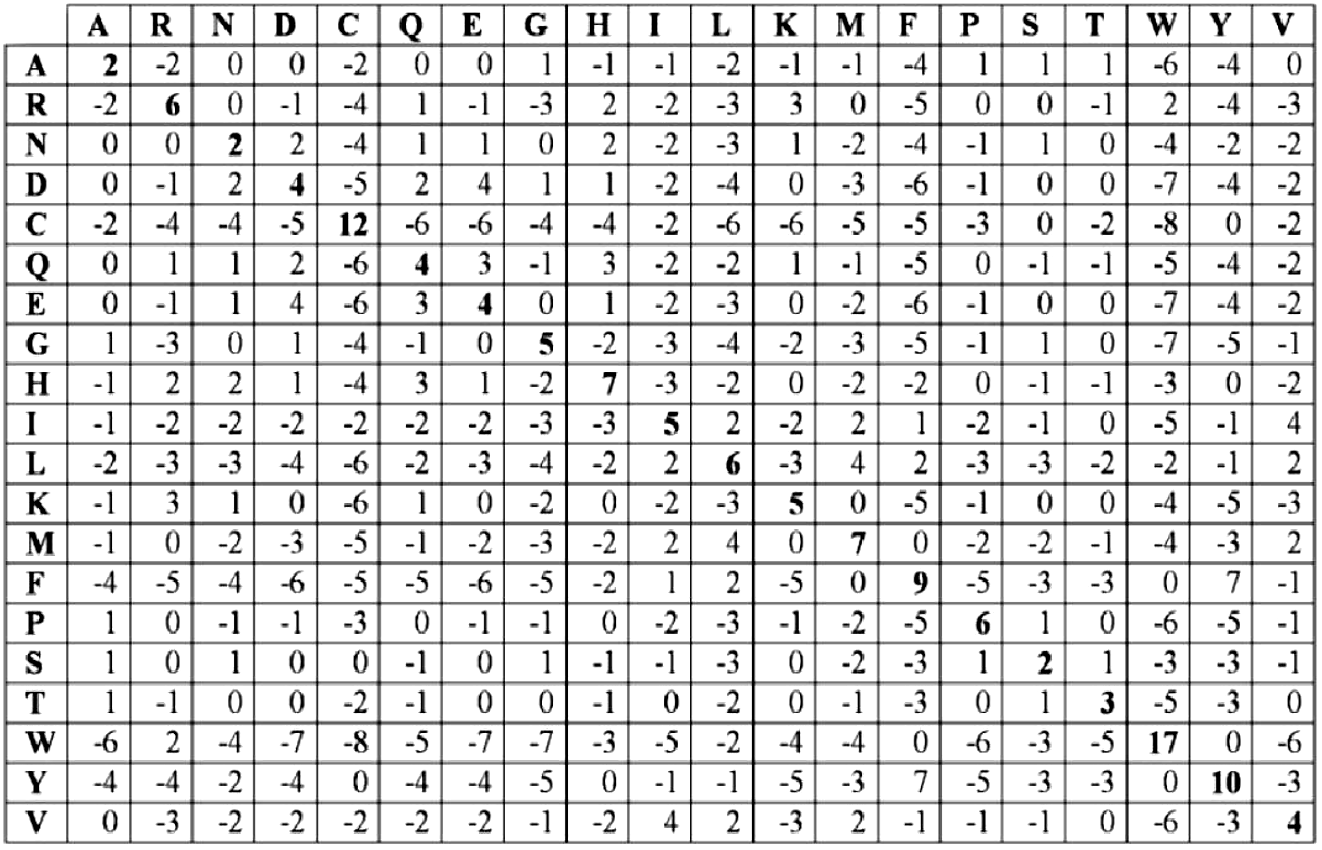
\includegraphics[scale=0.3]{PAM240}
 \end{figure}

\end{Exercise}

\begin{Exercise} [
  title={DeBruijn assembly},
  difficulty={2},
  label={exA},
  origin={G. Valle}
 ]

We want to discover the sequence of a hypothetical very small single stranded
genome, with an estimated length of 20 bases.

For this purpose, the 19 shotgun reads listed below were produced.

Unfortunately, the sequencing technology was not very good and some sequencing
errors may be possible.

You should attempt to assemble the genome with the DeBruijn graph method,
using \textbf{kmers of 4 bases}.

Consider that there are 256 different kmers of 4 bases.

\begin{verbatim}
Reads:
AACTTCTA
ACCTGATT
ACTTCTAC
ATTTCGGG
CCTGATTT
CGGGAACT
CTACCTGA
CTGATTTT
CTTCTACC
GAACTTCT
GATTTCGG
GGAACTTC
TACCTGAT
TCGGGAAC
TCTACCTG
TGATTTCG
TTCGGGAA
TTCTACCT
TTTCGGGG
\end{verbatim}


  \Question You should check if all the kmer occur more or less at the expected
level and you should consider possible repeated regions or kmers arising from
sequencing errors.

  \Question You should draw and analyse the resulting graph to establish if
there is one or more Eulerian cycles and if there is any evidence to establish
whether the original genome was linear or circular.

  \Question You should write the final circular genomic sequence.

Finally, you can further think about the peculiarity of this genome and why
DeBruijn graph are used, instead than full length reads.
\end{Exercise}


\newpage

\begin{Answer} [
  ref={exSW},
  number={4}
 ]

 The scoring matrix obtained by applying the algorithm is the following:

 \begin{figure}[H]
  \centering
  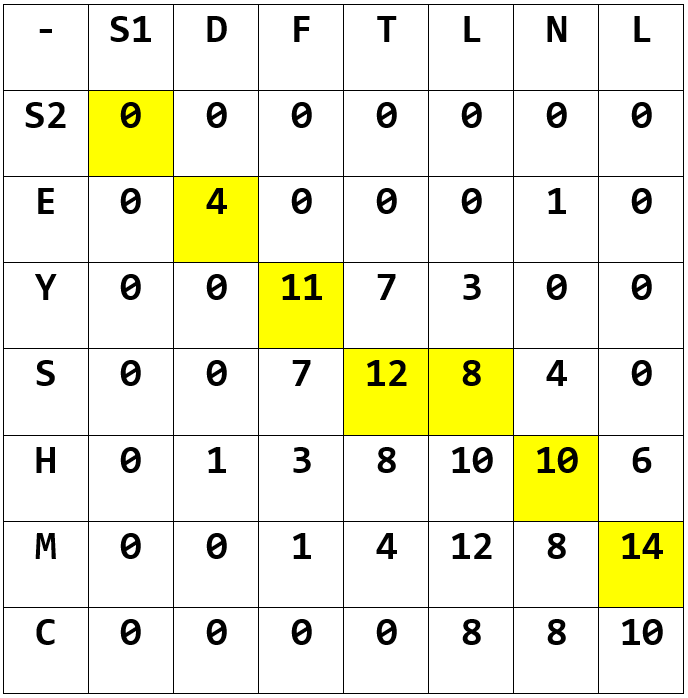
\includegraphics[scale=0.3]{matrix_ex}
 \end{figure}

 The \textbf{final alignment} is:

 \begin{figure}[H]
  \centering
  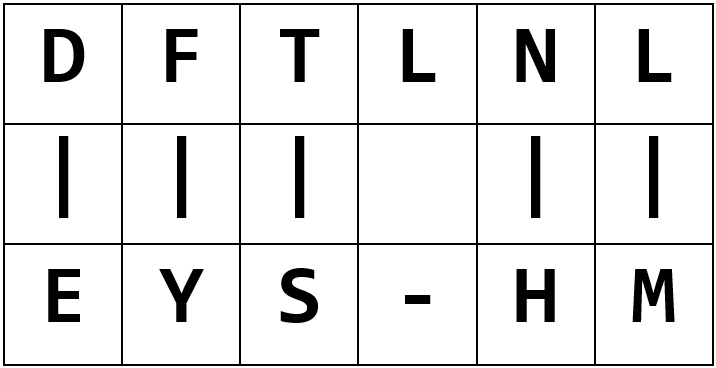
\includegraphics[scale=0.2]{alignment_ex}
 \end{figure}

 Thus, the \textbf{final score} is 14.

\end{Answer}

\begin{Answer} [
  ref={exA},
  number={6}
 ]

  \Question

\begin{tabular}{ | l | r | }
  \hline
  \textbf{Kmer} & \textbf{Count} \\ \hline
  \texttt{AACT} & 4 \\ \hline
  \texttt{ACTT} & 4 \\ \hline
  \texttt{ACCT} & 5 \\ \hline
  \texttt{ATTT} & 5 \\ \hline
  \texttt{CTTC} & 5 \\ \hline
  \texttt{CCTG} & 5 \\ \hline
  \texttt{CTGA} & 5 \\ \hline
  \texttt{CTAC} & 5 \\ \hline
  \texttt{CGGG} & 5 \\ \hline
  \texttt{TTCT} & 5 \\ \hline
  \texttt{TCTA} & 5 \\ \hline
  \texttt{TGAT} & 5 \\ \hline
  \texttt{TTTC} & 4 \\ \hline
  \texttt{TTCG} & 5 \\ \hline
  \texttt{TCGG} & 5 \\ \hline
  \texttt{TACC} & 5 \\ \hline
  \texttt{TTTT} & 1 \\ \hline
  \texttt{GATT} & 5 \\ \hline
  \texttt{GGGA} & 3 \\ \hline
  \texttt{GGAA} & 4 \\ \hline
  \texttt{GAAC} & 4 \\ \hline
  \texttt{GGGG} & 1 \\ \hline
\end{tabular}

Pheraps the kmers \texttt{TTTT} and \texttt{GGGG} should be considered as
sequencing errors.\footnote{
This script will help you to found all the kmers repetition:
\lstinputlisting[language=Bash]{res/code/assembly.sh}
You have to change launch the script with \textit{./script.sh /path/to/reads}.
Please pay attention that if there are 2 match in the same line one will be
counted out.}


  \Question \textbf{There is only one eulerian cycle}
\begin{figure}[H]
  \centering
  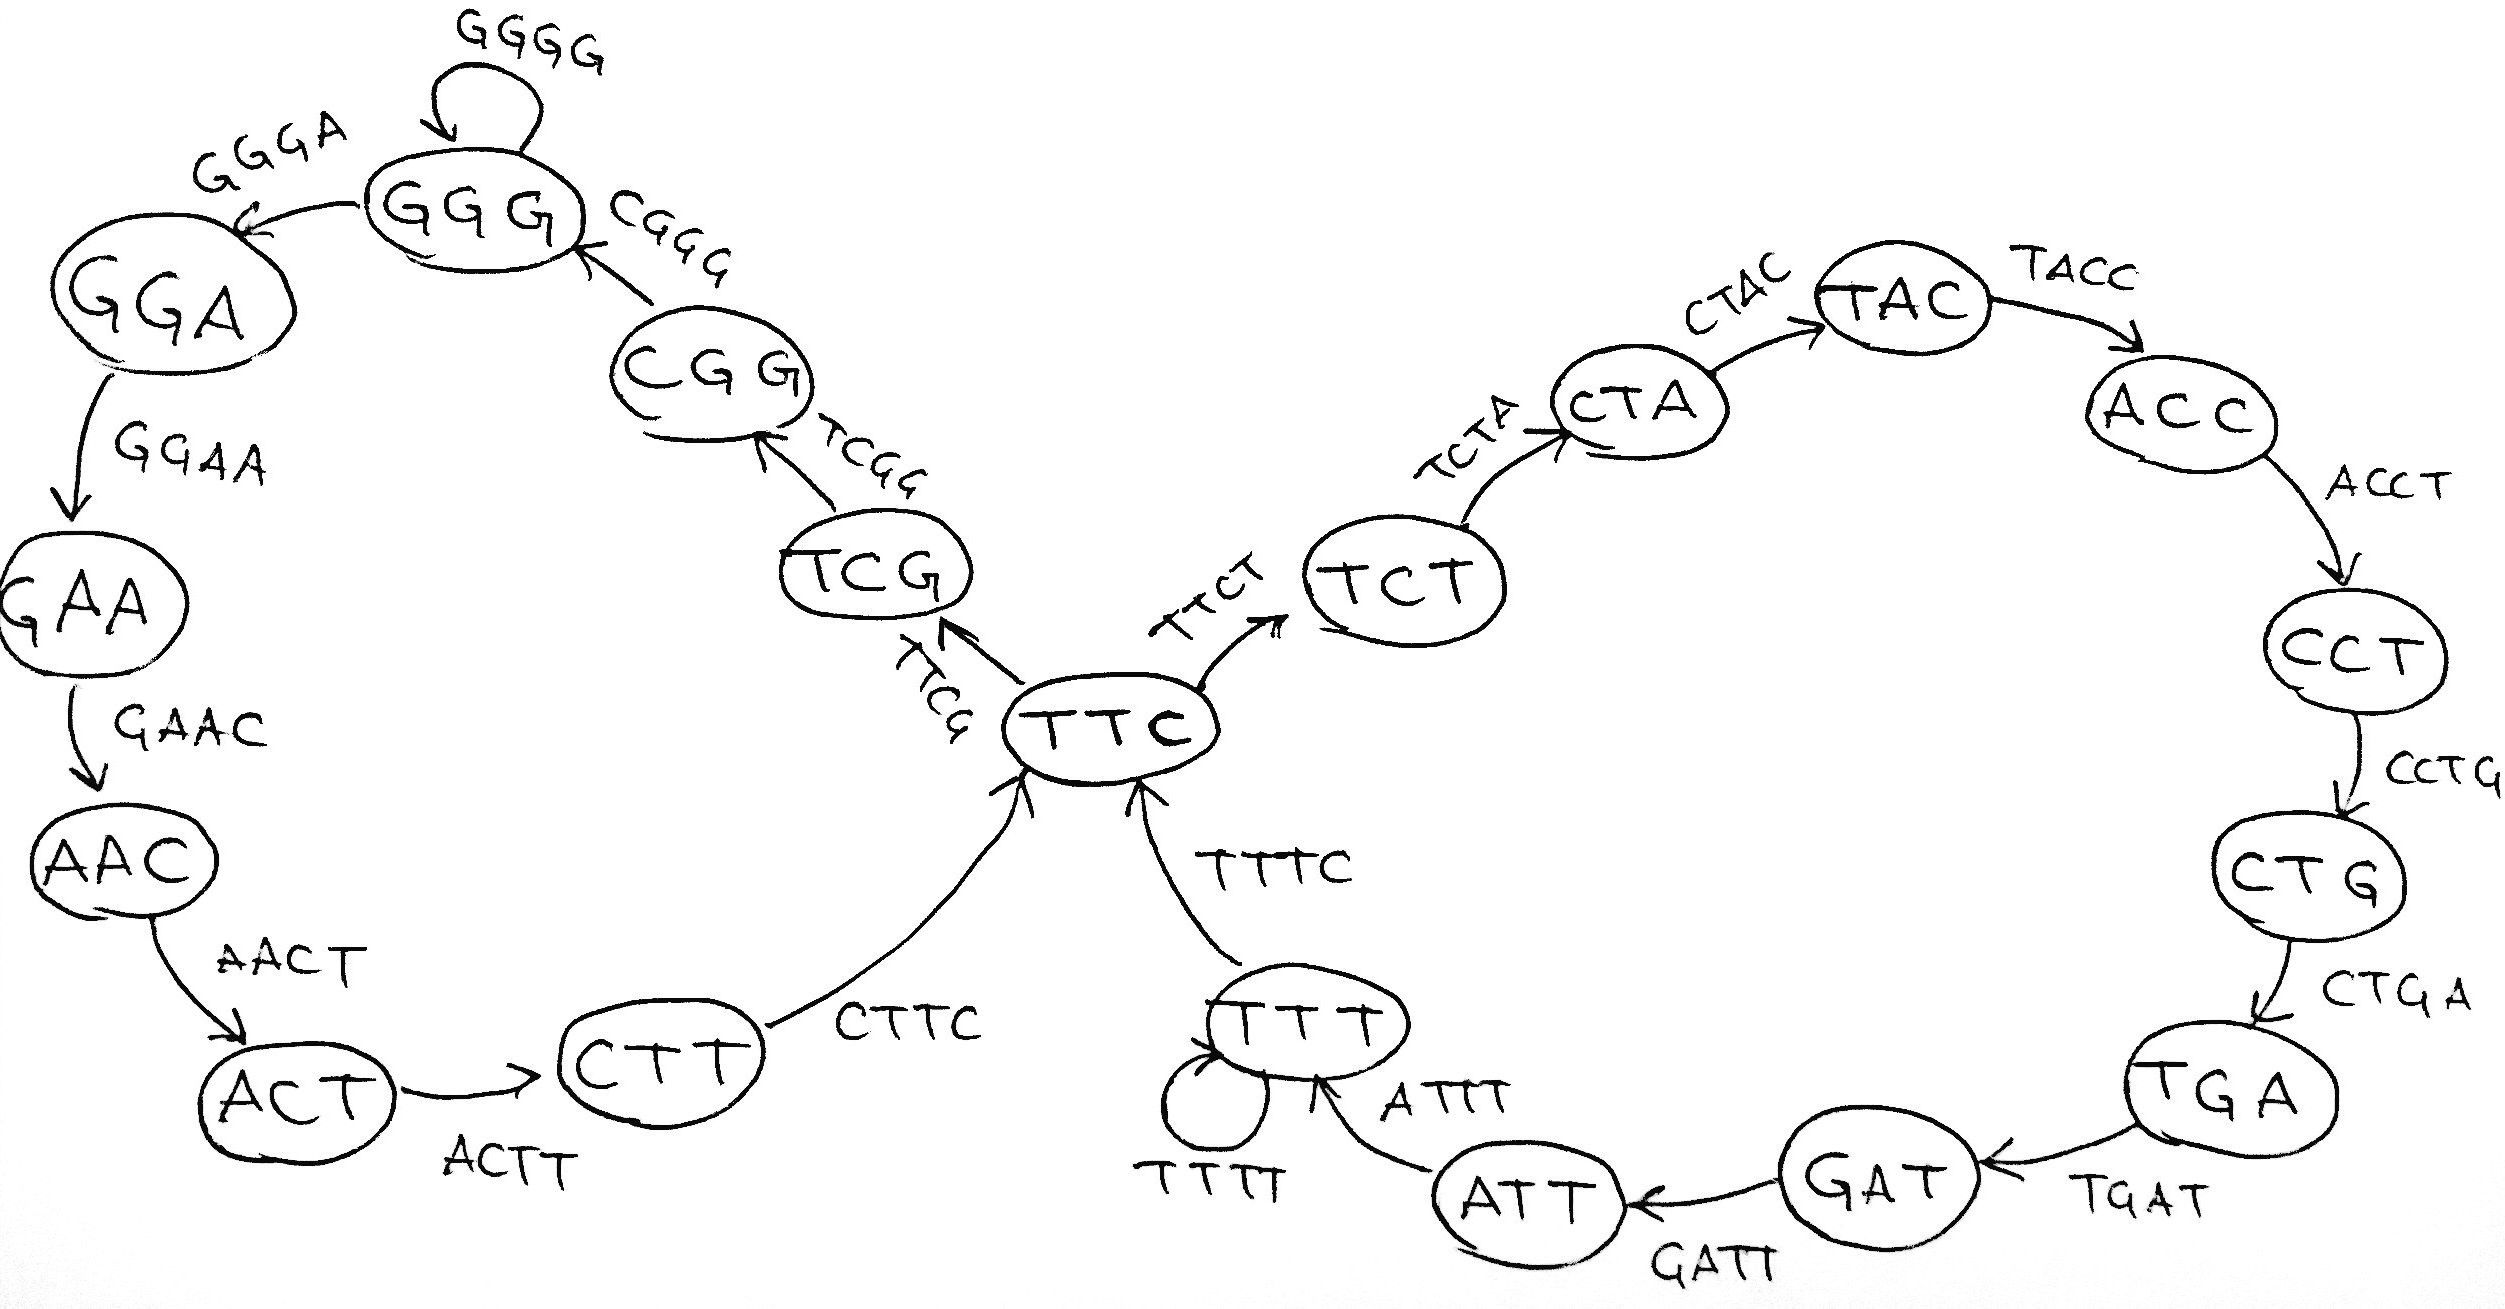
\includegraphics[scale=0.18]{graphA}
  \caption{graph}
\end{figure}

  \Question \texttt{{\color{red} TTC}TACCTGAT{\color{red} TTC}GGGAAC}
\end{Answer}

\section{Quiz}

\subsection{Flow of the genetic information}

\begin{Exercise} [
  title={Mitosis},
  difficulty={1},
  label={ex7},
  origin={G. Valle}
 ]

Answer \textbf{True} or \textbf{False}:

  \Question Mitosis is a process essential in the duplication of genetic
information of somatic cells.
Typically a diploid cell (2N) duplicates its DNA to become 4N, then the
chromosomes separate in two daughter diploid cells.

\end{Exercise}

\begin{Exercise} [
  title={Meiosis},
  difficulty={1},
  label={ex8},
  origin={G. Valle}
 ]

  \Question When we talk about DNA content in an eukaryotic cell, we refer to
N to indicate the DNA content.
Therefore we say that a haploid cell is 'N' and a diploid cell is '2N'.

Meiosis is a process essential in distributing genetic information in germinal
cells. What happens during  meiosis?

Choose an alternative:

\begin{enumerate}
  \item During meiosis,  a diploid cell (2N) duplicates its DNA to become 4N,
then there are two cell divisions without DNA duplication, producing 4 haploid
cells called “gametes”, each with N chromosomes.
  \item The entire process of meiosis starts from a diploid cell (2N) that
divides itself into two haploid cells (N) called “gametes”, each with N
chromosomes.
\end{enumerate}

\end{Exercise}

\begin{Exercise} [
  title={Crossing-Over (1)},
  difficulty={1},
  label={ex9},
  origin={G. Valle}
 ]

Answer \textbf{True} or \textbf{False}:

  \Question Crossing over is a genetic process that is important in evolution
because it creates new mutations

\end{Exercise}

\begin{Exercise} [
  title={Crossing-Over (2)},
  difficulty={1},
  label={ex10},
  origin={G. Valle}
 ]

  \Question When does crossing over occurs?

Choose an alternative:

\begin{enumerate}
  \item It occurs during mitosis.
  \item It occurs during meiosis.
  \item It occurs at every cell duplication.
\end{enumerate}

\end{Exercise}

\begin{Exercise} [
  title={Eukaryotes},
  difficulty={1},
  label={ex11},
  origin={G. Valle}
 ]

Answer \textbf{True} or \textbf{False}:

  \Question Eukaryotes alternate haploid and diploid generations

\end{Exercise}

\begin{Exercise} [
  title={Haploidy},
  difficulty={1},
  label={ex12},
  origin={G. Valle}
 ]

Answer \textbf{True} or \textbf{False}:

  \Question The haploid status is predominant in most eukaryotes

\end{Exercise}

\begin{Exercise} [
  title={Diploidy},
  difficulty={1},
  label={ex13},
  origin={G. Valle}
 ]

Answer \textbf{True} or \textbf{False}:

  \Question Diploidy is important in evolution because it helps to eliminate
bad genes.

\end{Exercise}

\subsection{Answers (Flow of the genetic information)}

\begin{Answer} [
   ref={ex7},
   number={7}
 ]

  \Question \textbf{True}

\end{Answer}

\begin{Answer} [
   ref={ex8},
   number={8}
 ]

  \Question 1

Typically, during meiosis,  a diploid cell (2N) duplicates its DNA to become
4N, then there are two cell divisions without DNA duplication, producing 4
haploid cells called “gametes", that are 1N.

\end{Answer}

\begin{Answer} [
   ref={ex9},
   number={9}
 ]

  \Question \textbf{False}

\end{Answer}

\begin{Answer} [
   ref={ex10},
   number={10}
 ]

  \Question 2

\end{Answer}

\begin{Answer} [
   ref={ex11},
   number={11}
 ]

  \Question \textbf{True}

It is true. For instance in mammals, there is the alternation between the
diploid phase (that is hugely predominant and multicellular) with the haploid
stage that is unicellular, represented by the egg and the spermatozoon.
The two haploid gametes join during fertilization to produce a diploid cell
that by means of many cell duplications (mitosis) will generate the fully
developed diploid organism.
Some specialized organs (gonads) are responsible to host the process of
gametogenesis where the haploid gametes are produced by meiosis.

\end{Answer}

\begin{Answer} [
   ref={ex12},
   number={12}
 ]

  \Question \textbf{False}

\end{Answer}

\begin{Answer} [
   ref={ex13},
   number={13}
 ]

  \Question \textbf{False}

\end{Answer}

\subsection{DNA Sequencing}

\begin{Exercise} [
  title={NGS},
  difficulty={1},
  label={ex14},
  origin={G. Valle}
 ]

Answer \textbf{True} or \textbf{False}:

  \Question There are several technologies for DNA sequencing.
The so called Next Generation Sequencing technologies, like Illumina, are able
to produce hundreds of million reads, but only from very short fragments of
DNA, a few hundred bases long.

\end{Exercise}

\begin{Exercise} [
  title={Sanger Sequencing},
  difficulty={1},
  label={ex15},
  origin={G. Valle}
 ]

Answer \textbf{True} or \textbf{False}:

  \Question The Sanger sequencing technology has been very important in the
past, but now is obsolete and the Sanger DNA sequencers are not anymore
available on the market.

\end{Exercise}

\begin{Exercise} [
  title={DNA Analysis},
  difficulty={1},
  label={ex16},
  origin={G. Valle}
 ]

A DNA locus has been sequenced both from father and mother.
The results show that one base is different (shown by the arrow).

 \begin{figure}[H]
  \centering
  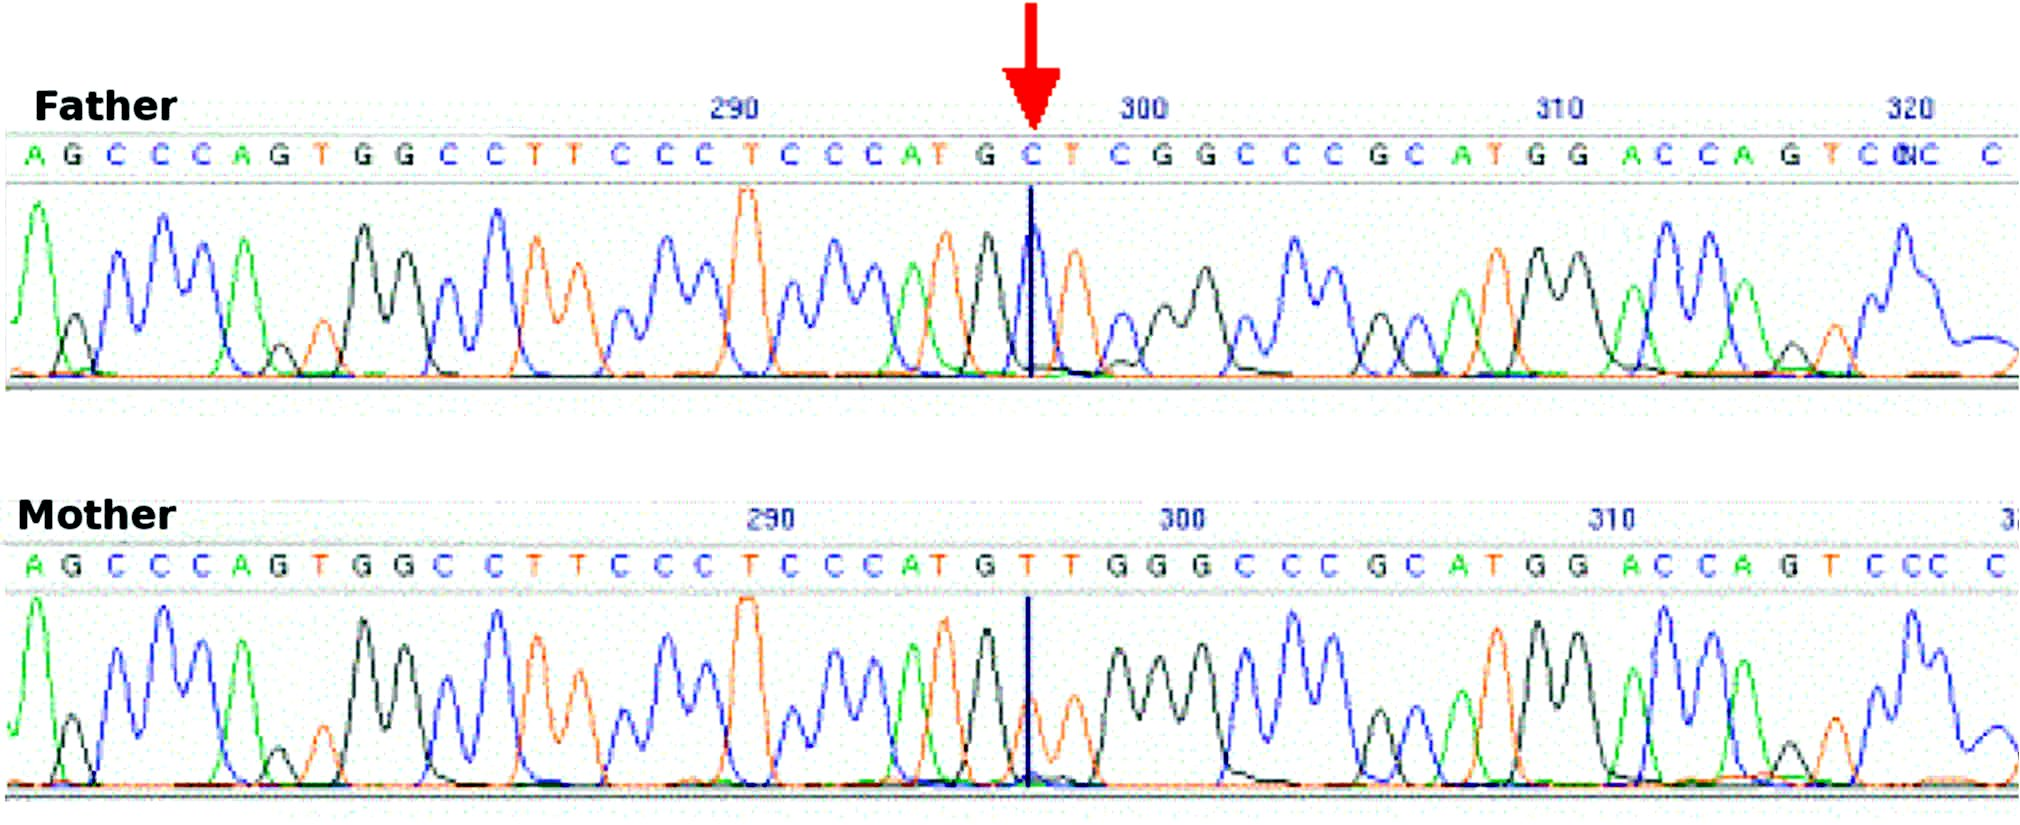
\includegraphics[scale=0.2]{sanger1}
 \end{figure}

Choose an alternative:

\begin{enumerate}
  \item Both father and mother are homozygous.
  \item Both father and mother are heterozygous.
  \item Their child will be heterozygous.
  \item Their child will be homozygous.
  \item The child could be either homo or heterozygous depending on the
chromosomal re-assortment.
\end{enumerate}

\end{Exercise}

\begin{Exercise} [
  title={Sequence coverage},
  difficulty={1},
  label={ex17},
  origin={G. Valle}
 ]

  \Question A genome of 5 million bases (5 Mbp) has been shotgun sequenced
using mate pair reads.

The DNA fragments average 10000 bp and the reads average 500 bases.
A total of 10000 reads were produced (5000 pairs). Estimate the average
\textbf{sequence coverage}.

\end{Exercise}

\begin{Exercise} [
  title={Physical coverage},
  difficulty={1},
  label={ex18},
  origin={G. Valle}
 ]

  \Question A genome of 5 million bases (5 Mbp) has been shotgun sequenced
using mate pair reads.

The DNA fragments average 10000 bp and the reads average 500 bases.
A total of 10000 reads were produced (5000 mates pairs). Estimate the average
\textbf{physical coverage}.

\end{Exercise}

\begin{Exercise} [
  title={Mate pairs},
  difficulty={1},
  label={ex19},
  origin={G. Valle}
 ]

A mate pairs library was sequenced and mapped on a reference genome.
The 3 tracks shown in the figure show a particular region of the genome.
What do you think is there?

 \begin{figure}[H]
  \centering
  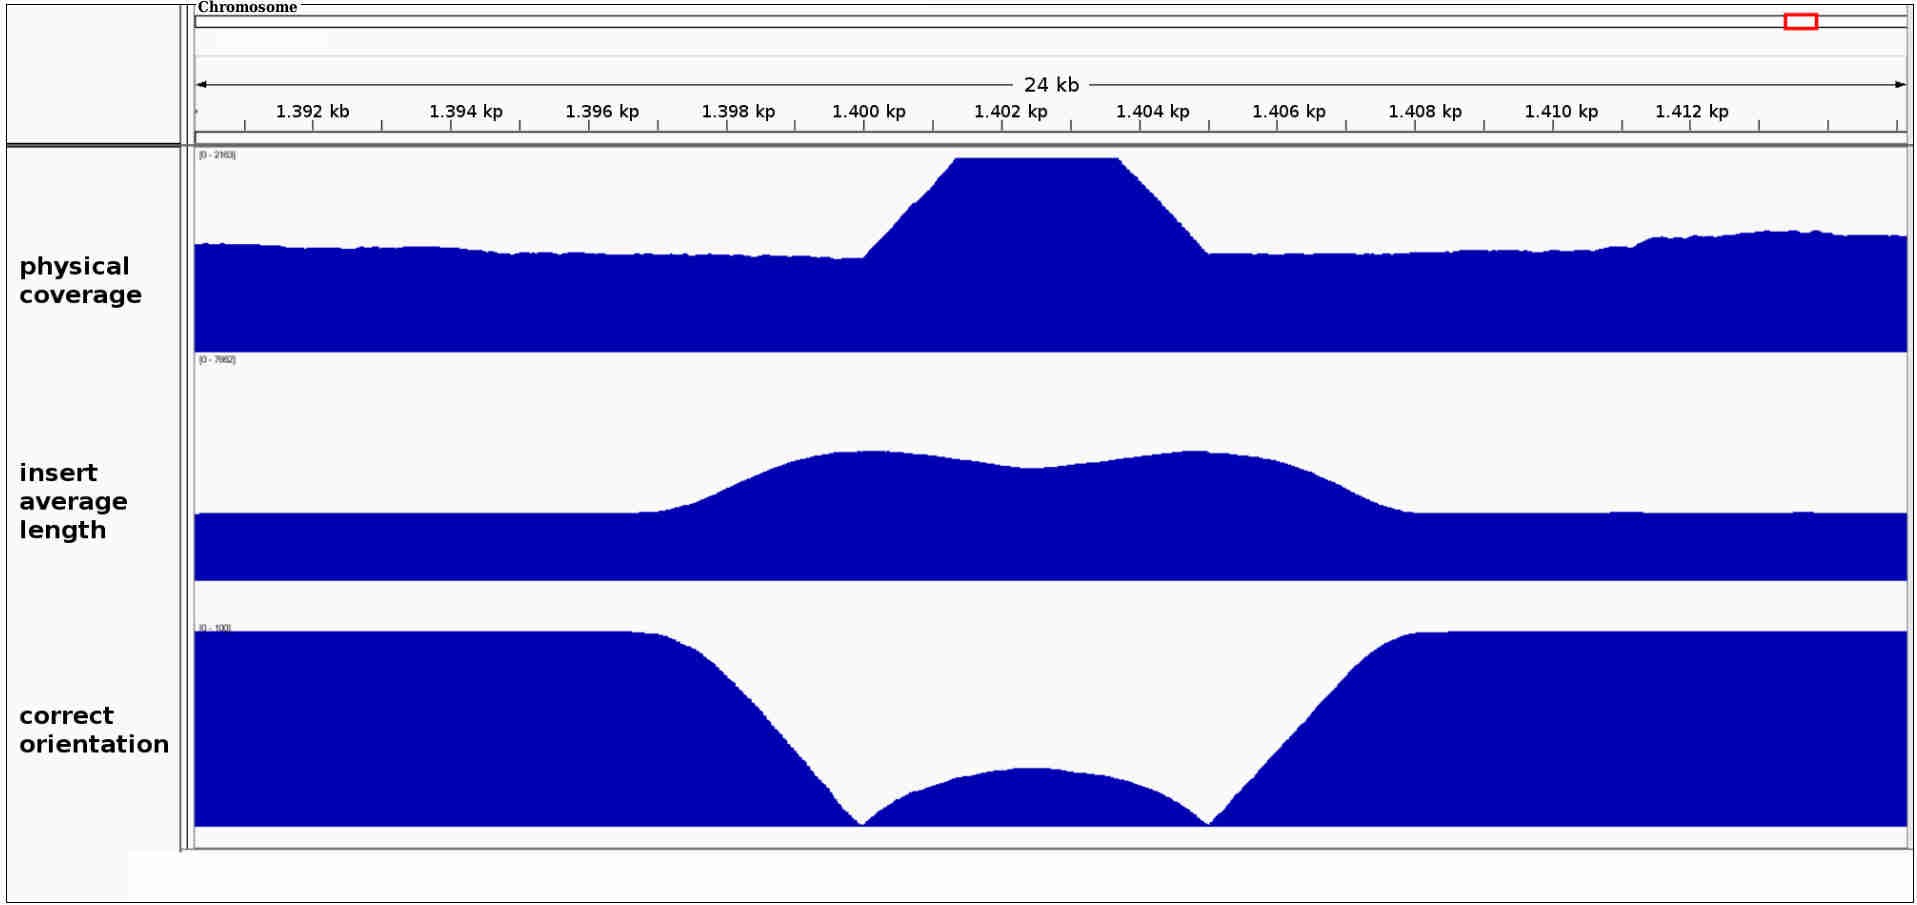
\includegraphics[scale=0.2]{tracks}
 \end{figure}

Choose an alternative:

\begin{enumerate}
  \item long deletion.
  \item short deletion.
  \item long insertion.
  \item long inversion.
  \item short insertion.
  \item short inversion
\end{enumerate}

\end{Exercise}

\subsection{Answers (DNA Sequencing)}

\begin{Answer} [
   ref={ex14},
   number={14}
 ]

  \Question \textbf{True}

\end{Answer}

\begin{Answer} [
   ref={ex15},
   number={15}
 ]

  \Question \textbf{False}

Sanger sequencing is still very important and there are still Sanger DNA
sequencers on the market.

For instance, if you want to sequence a short piece of DNA, you don't need
million reads!

Furthermore, there are many DNA sequencing services that will do everything
for you: you supply the DNA, for instance a fragment amplified by PCR, and
they give you the sequence at a cost of less than 5 euro.

\end{Answer}

\begin{Answer} [
   ref={ex16},
   number={16}
 ]

  \Question 1,3

In the case of heterozygosity we would see two different color peaks
overlapping as shown below.
Instead we see that at the given locus the father shows a C and the mother
a T, both in homozygosity.
The father will pass to the child the C allele and the mother the T allele.
Therefore the child will be certainly heterozygous carrying both alleles.

The correct answer is \textbf{Both father and mother are homozygous,
their child will be heterozygous}

\end{Answer}

\begin{Answer} [
   ref={ex17},
   number={17}
 ]

  \Question 1

\textbf{Formula} The average coverage for a whole genome can be calculated
from the length of the original genome (G), the number of reads (N), and the
average read length (L) as $N*L/G$

\end{Answer}

\begin{Answer} [
   ref={ex18},
   number={18}
 ]

  \Question 10\footnote{Protip: the sequence coverage can't be greater than the
physical coverage.}

\textbf{Formula} The formula is: $P*F/G$ where:
\begin{itemize}
 \item P is the number of mate pairs
 \item F is the avarage fragment length
 \item G is the length of the original genome
\end{itemize}

\end{Answer}

\begin{Answer} [
   ref={ex19},
   number={19}
 ]

  \Question 4 (long inversion)

\end{Answer}

\subsection{Others questions}

\begin{Exercise} [
  title={mRNA},
  difficulty={1},
  label={ex20},
  origin={G. Valle}
 ]

Answer \textbf{True} or \textbf{False}:

  \Question The mature mRNA is encoding proteins by means of codons that are
3 bases long. Therefore mRNA have lengths that are necessarily multiple of 3.

\end{Exercise}

\begin{Exercise} [
  title={Splicing},
  difficulty={1},
  label={ex21},
  origin={G. Valle}
 ]

Answer \textbf{True} or \textbf{False}:

  \Question Many genes contain introns that must be removed to obtain a
functional mRNA (splicing process).
The splicing mechanism is performed by the enzyme RNA polymerases that
recognizes the introns and transcribes into mRNA only the exons.
As a result the mRNA is constituted only by the exons.

\end{Exercise}

\begin{Exercise} [
  title={Objective function for alignment},
  difficulty={1},
  label={ex22},
  origin={G. Valle}
 ]

\begin{equation}
Score = \sum_{i=1}^{L} s(a_i,b_i) - \sum_{j=1}^{G} (\gamma + \delta(len(j)-1))
\end{equation}

  \Question Explain what these symbols represent: L, G, $\gamma$, $\delta$,
$s(a_i,b_i)$

\end{Exercise}

\subsection{Others answers}

\begin{Answer} [
   ref={ex20},
   number={20}
 ]

  \Question \textbf{False}

Although the coding regions have a length that must be multiple of 3, there are untranslated regions both in 3' and 5' (respectively 3'UTR and 5'UTR) that can be any length. Therefore the mRNA is not necessarily a multiple of 3.

\end{Answer}

\begin{Answer} [
   ref={ex21},
   number={21}
 ]

  \Question \textbf{False}

RNA polymerases transcribe into RNA the full length of a gene, including the introns. The splicing process acts on the transcribed RNA by removing the intronic portions.

\end{Answer}

\begin{Answer} [
   ref={ex22},
   number={22}
 ]

  \Question L – length of the alignment, $\delta$ – penalty for gap elongation,
G – number of gaps, $\gamma$ – penalty for staring a gap, $s(a_i, b_i)$ –
score of the match at position i.

\end{Answer}

\subsection{Sequencing}

\begin{Exercise} [
  label={ex23},
  origin={G. Valle}
 ]

\begin{figure}[H]
  \centering
  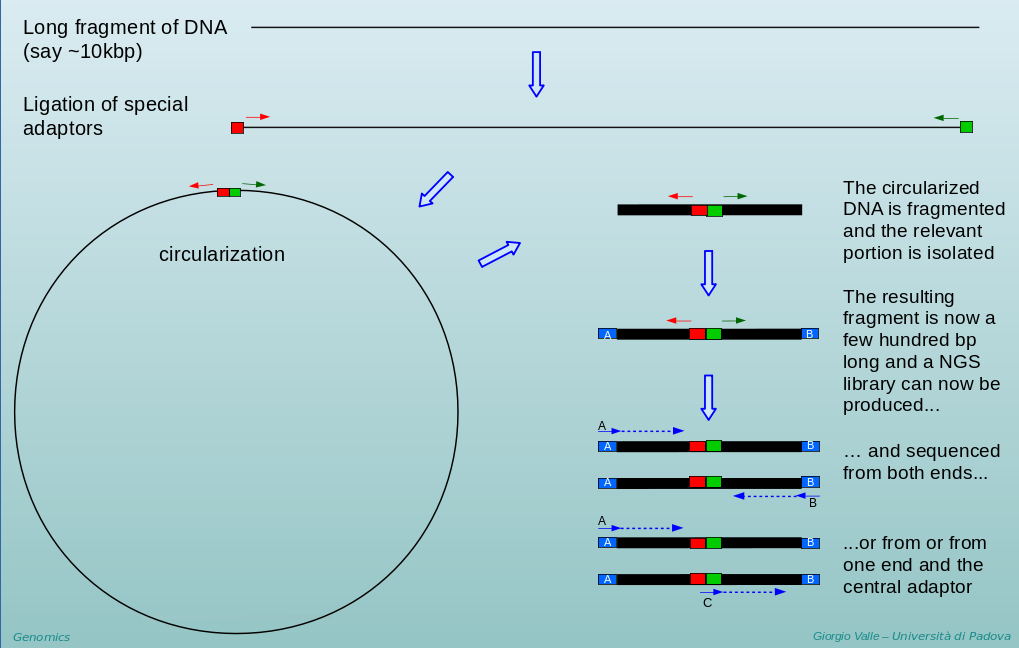
\includegraphics[scale=0.3]{matepairsex}
\end{figure}

The figure shows the main steps for the construction of a mate pair library.
Two reads will be obtained from each insert. The two reads will map on the
genome on the forward strand (F) or on the reverse strand (R). Thus, each mate
pair will have one of these combinations: FF, RR, FR, RF, where the first
letter corresponds to the read mapping before (towards the 5' end) in the
reference genome and the second letter corresponds to the ``mate'' read  mapping
after (i.e. towards the 3' end).

Choose one or more answers:

\Question If the sequencing is done with primers A and C, do you need to attach
the adaptor B ?
\begin{enumerate}
\item Yes
\item It depends
\item No
\end{enumerate}

\Question Which direction do you expect if the reads are produced with primers
A and B (see figure)
\begin{enumerate}
\item RR
\item FF
\item RF
\item FR
\end{enumerate}

\Question Which direction do you expect if the reads are produced with primers
A and C (see figure)
\begin{enumerate}
\item FF
\item RR
\item RF
\item FR
\end{enumerate}

\end{Exercise}

\begin{Answer} [
  ref={ex23},
  number={1}
 ]

\Question Yes
\Question RF
\Question FR

\end{Answer}

\begin{Exercise} [
  label={ex24},
  origin={G. Valle}
 ]

\Question Reconstruct the process of de novo assembly alternating an activity
and an entity.
\begin{itemize}
\item MATE PAIRS ALIGNMENT
\item FASTQ FILE
\item VALIDATION
\item SCAFFOLDS
\item OVERLAP ASSEMBLY
\item LIBRARY
\item CONTIGS
\item SEQUENCING
\item DRAFT GENOME
\end{itemize}

\end{Exercise}

\begin{Answer} [
  ref={ex24},
  number={1}
 ]

\Question 
\begin{enumerate}
\item LIBRARY
\item SEQUENCING
\item FASTQ FILE
\item OVERLAP ASSEMBLY
\item CONTIGS
\item MATE PAIRS ALIGNMENT
\item SCAFFOLDS
\item VALIDATION
\item DRAFT GENOME
\end{enumerate}

\end{Answer}

\begin{Exercise} [
  label={ex25},
  origin={G. Valle}
 ]

Imagine that you have assembled a genome into contigs and you want to further
assemble your contigs into scaffolds. Given the cases described below, select
the corresponding methods that you think are suitable, from this list:
\begin{enumerate}
\item Optical mapping
\item Genetic maps
\item Comparative genome analysis
\item BAC-end sequencing
\item Radiation hybrids
\item PacBio sequencing, to produce very long reads
\item Mate pairs
\item BAC fingerprinting + BAC-end sequencing
\item BAC Fingerprinting
\end{enumerate} 

\Question The genome belongs to a plant with a large genome that is
phylogenetically distant from any other plant with known genome

\Question The genome belongs to a bacterium with a relatively small genome

\Question It is a mammalian genome and a BAC library is available

\end{Exercise}

\begin{Answer} [
  ref={ex25},
  number={1}
 ]

\Question Plant genome phylogenetically distant: this will be difficult.
Optical mapping could be an option, but it is still poorly exploited and it
works only for genomes that are not too long. PacBio could also be an option,
as well as mate pairs sequencing\\\textbf{Optical mapping}

\Question Bacterial genome: should be much easier. mate pairs should be a good
approach\\\textbf{Mate pairs}

\Question Mammalian genome with BAC library: To do BAC-end sequencing and/or
BAC fingerprinting is too expensive. Try to calculate how any Sanger runs you
would need. Since there are many mammalian genomes available, a better choice
would be the comparative genome analysis, possibly considering several
mammalian genomes\\\textbf{Comparative genome analysis}

\end{Answer}

\begin{Exercise} [
  label={ex26},
  origin={G. Valle}
 ]

Complete the sentence below with 3 of these words:
\begin{itemize}
\item Eulerian
\item Hamiltonian
\item path
\item bridge
\item circle
\item linear
\item circular
\item fragmented
\end{itemize}

A sequence was analysed for its kmer content and as a result this graph was
obtained.

\begin{figure}[H]
  \centering
  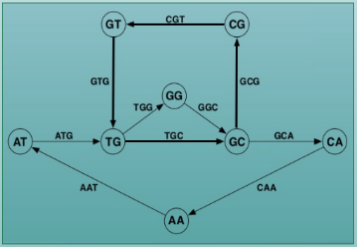
\includegraphics[scale=0.5]{circle}
\end{figure}

\Question From the graph we understand that a (a) (b) can be obtained,
therefore the genome is (c)

\end{Exercise}

\begin{Answer} [
  ref={ex26},
  number={1}
 ]

\Question (a)Eulerian \\(b)circle \\(c)circular\\
From the graph we understand that a \textbf{Eulerian} \textbf{circle} can be
obtained, therefore the genome is \textbf{circular}

\end{Answer}

\begin{Exercise} [
  label={ex27},
  origin={G. Valle}
 ]

\Question This question is about "Bridge PCR". The amplification in this case
occurs on a plain structure, often called "flowchip". Is it true that only one
of the two PCR primers is bound to the flowchip, while the other primer is free
in the solution?

\end{Exercise}

\begin{Answer} [
  ref={ex27},
  number={1}
 ]

\Question No

\end{Answer}

\begin{Exercise} [
  label={ex28},
  origin={G. Valle}
 ]

\Question Which DNA sequencers use methods based on emulsionPCR?
Choose one or more answers:
\begin{enumerate}
\item PacBio
\item SOLiD
\item Oxford Nanopore
\item Illumina
\item Pyrosequencing (454 Roche)
\item Ion Proton
\item Sanger
\end{enumerate}

\end{Exercise}

\begin{Answer} [
  ref={ex28},
  number={1}
 ]

\Question Ion Proton, SOLiD, Pyrosequencing (454 Roche)

\end{Answer}

\begin{Exercise} [
  label={ex29},
  origin={G. Valle}
 ]

\Question Which components do you have to include in the emulsion PCR mixture?
Scegli una o più alternative:
\begin{enumerate}
\item mRNA
\item dNTPs
\item tRNA
\item Primers
\item Taq Polymerase
\item NGS library
\item ATP
\item SDS
\end{enumerate}

\end{Exercise}

\begin{Answer} [
  ref={ex29},
  number={1}
 ]

\Question dNTPs, Taq Polymerase, Primers, NGS library

\end{Answer}

\begin{Exercise} [
  label={ex30},
  origin={G. Valle}
 ]

From a genome 60 million bases long, we produced a mate-pair library with
inserts averaging 6000 bp, with a standard deviation of 500 bases, then we made
an Illumina NGS library and we produced 20 million mate pairs 150+150 bases 
i.e. 20 million forward and 20 million reverse).

\Question Calculate the average sequence coverage

\Question Calculate the average physical coverage

\Question How much do you think it costs to produce the 6 billion bases for
this experiment?  Give your estimate number of Euro

\end{Exercise}

\begin{Answer} [
  ref={ex30},
  number={1}
 ]

Sequence coverage:
150 bases x 40 millions = 6 billions bases produced by the DNA sequencer
6 billions / 60 million = 100 average sequence coverage

Physical coverage:
Each mate pair produces 150+150 bases = 300 bases of sequence
Each mate pair produces 6000 bases of physical coverage
the physical coverage will be 6000/300 = 20 times more than sequence coverage
Therefore physical coverage = 2000

The accuracy of predicting an insertion/deletion of 300 bases will be high
because although the standard deviation is 600, you must take into account that
there will be about 2000 fragments covering that position. Therefore you must
calculate that the standard deviation of a population of 2000 cases must be
divided by the square root of 2000, that is $\sim$45. Thus 600/45 = 13.4 bases

A coverage of 100x is suitable for a genomic sequencing project
The cost of reagents to produce 6 billion bases on Illumina could be $\sim$
\euro 300

\Question 100

\Question 2000

\Question \euro 300

\end{Answer}

\begin{Exercise} [
  label={ex31},
  origin={G. Valle}
 ]

\Question Assume that the genome that you are sequencing has a sequence of 300
bases that is tandem repeated 6 times, while in the reference genomes it is
repeated 5 times. Would you be able to predict whether there are 5 or 6 repeats?
\begin{itemize}
\item Yes, with an accuracy >90\%
\item We could only make a low accuracy hypothesis if we knew a priory that
there may be a difference
\item No, because the difference of 300 bases is too small when the standard
deviation is 600 bases
\end{itemize}


\end{Exercise}

\begin{Answer} [
  ref={ex31},
  number={1}
 ]

\Question Yes, with an accuracy >90\%

\end{Answer}

\begin{Exercise} [
  label={ex32},
  origin={G. Valle}
 ]

\Question What is the expected percentage of the genome covered exactly by 3
reads? (Approximate to the nearest integer)

\Question What is the expected percentage of the genome still uncovered by
reads? (Approximate to the nearest integer)
\end{Exercise}

\begin{Answer} [
  ref={ex32},
  number={1}
 ]

\Question  You must consider the Poisson distribution with v=3 and r=2:
\begin{equation}
f(v) = \frac{e^{-r}*r^v}{v!} \sim \frac{2.7^{-2}*2^3}{3!} \sim 
\frac{0.14 * 8}{6} \sim 0.18
\end{equation}
Therefore $\sim$18\% of the genome will be covered by 3 reads

\Question To do a precise calculation you should consider the poisson formula,
or its simplified version for v=0 (that is for the probability that a position
is covered 0 times). That is e to the power -r, where r is the ``redundancy''
that is the average coverage. In our case r=2, therefore:
\begin{equation}
e^{-2} = \frac{1}{e^2} \sim \frac{1}{2.7^2} \sim \frac{1}{7} \sim 0.14
\end{equation}
Therefore, about 14\% of the genome is expected to be uncovered by reads
\end{Answer}

\begin{Exercise} [
  label={ex33},
  origin={G. Valle}
 ]

\Question Consider this formula (where \textbf{e} is approximately equal to 2.7)
\begin{equation}
f(v) = \frac{e^{-r}*r^v}{v!}
\end{equation}
What is it about?
\end{Exercise}

\begin{Answer} [
  ref={ex33},
  number={1}
 ]

\Question  The formula is about the Poisson distribution 
\end{Answer}

\subsection{Genomic Assembly}

\begin{Exercise} [
  label={ex34},
  origin={G. Valle}
 ]
Prefix and suffix tree find useful applications in programs to align reads on a
reference genome.  Here is shown a prefix tree of the word GOOGOL.

\begin{figure}[H]
  \centering
  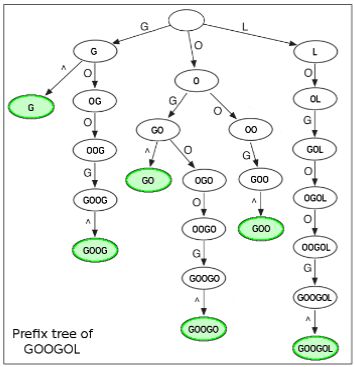
\includegraphics[scale=0.5]{googol}
\end{figure}

\Question Choose one or more answers:
\begin{enumerate}
\item With suitable algorithms and with the information contained in a prefix
tree like this, it is possible to find if any word is present in the genome
\item With suitable algorithms and with the information contained in a prefix
tree like this, it is possible to find also the position of the word in the
genome
\item With suitable algorithms and with the information contained in a prefix
tree like this, it is possible to find also similar words, not only perfect
matches
\item With the information contained in a prefix tree like this it is only
possible to know if a word exist in the genome, not how many times it occurs
\item A prefix tree like this it is also called Burrow-Weeler Transform
\item The program BWA uses prefix trees together with some indexes obtained by
the Burrow-Weeler
\end{enumerate}

\end{Exercise}

\begin{Answer} [
  ref={ex34},
  number={1}
 ]

\Question The right answers are:
\begin{itemize}
\item With suitable algorithms and with the information contained in a prefix
tree like this, it is possible to find if any word is present in the genome
\item The program BWA uses prefix trees together with some indexes obtained by
the Burrow-Weeler Transform algorithm
\end{itemize}

The first one is correct because all the words will be represented by nodes 
(including internal words, as it can be seen in the GOOGOL tree). Therefore, an
algorithm can go through the tree to see if the word is present. This is much
faster that going through the whole genome. It is like an index.  Differently
from algorithms based on "seed and extend", where the ``seeds'' (=kmers) have a
given length, a tree allows to index all the words of any length

\end{Answer}

\begin{Exercise} [
  label={ex35},
  origin={G. Valle}
 ]
The whole genome assembly of an organism produced the following set of contigs, ranging from 541 to 6100 bases.
\begin{figure}[H]
  \centering
  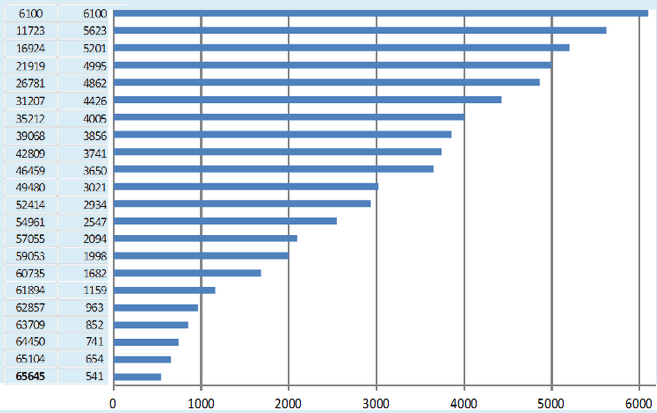
\includegraphics[scale=0.5]{lnvalue}
\end{figure}

\Question The organism that was sequenced is probably a:
\begin{enumerate}
\item Plant
\item Archea
\item Animal
\item Bacterium
\item Virus
\end{enumerate}

\Question The N50 value is:
\begin{enumerate}
\item 35212
\item 6
\item 12
\item 3650
\item 8
\item 46459
\item 9
\item 3021
\item 7
\item 11
\item 49480
\item 10
\item 32822
\item 4005
\item 22
\end{enumerate}

\Question The L50 value is:
\begin{enumerate}
\item 35212
\item 6
\item 12
\item 3650
\item 8
\item 46459
\item 9
\item 3021
\item 7
\item 11
\item 49480
\item 10
\item 32822
\item 4005
\item 22
\end{enumerate}

\end{Exercise}

\begin{Answer} [
  ref={ex35},
  number={1}
 ]

\Question Virus

\Question 4005

\Question 7

\end{Answer}

\begin{Exercise} [
  label={ex36},
  origin={G. Valle}
 ]

The chromosomes of many plants and animals are often more than 100
million bp, while our current DNA sequencing technology is only able to produce
relatively short reads of a few hundred bases. This is still a big problem if
we need to assemble a new genome.

Now, say that we performed a Whole Genome Shotgun of a Mollusc that does not
have phylogenetically related organism known at genomic level. We know that the
haploid genome is approximately 4 Gbp and we assume that it has an organization
(repeated sequences, chromosomes, introns, exons) similar to mammals.

In this example we consider that we have produced paired-end Illumina reads
100+100 bases long from genomic inserts of ~1000 bases, to achieve a sequence
coverage of 100x.

\Question How many individual reads of 100 bases are required?

\Question What is the resulting physical coverage?
\end{Exercise}

\begin{Answer} [
  ref={ex36},
  number={1}
 ]

\Question if the reads are 100 bases long and you need a 100x coverage, then
you will need on average one read per every base of the genome, no matter how
long is the genome. In this specific case, since the genome is 4 billion bases,
you will need 4 billion reads.\\
So the answer is \textbf{4000000000}

\Question Every read-pair has 2 reads of 100 bases (total 200 bases of reads
coverage) and 1000 bases of insert (i.e. 1000 bases of physical coverage).
Therefore the physical coverage will be 5 times greater than the sequence
coverage. Since the sequence coverage was 100x, the physical coverage will be
500x.\\
So the answer is \textbf{500}
\end{Answer}

\begin{Exercise} [
  label={ex37},
  origin={G. Valle}
 ]

\Question After the assembly of the reads with Velvet (that is a program based
on DeBruijn graphs), what is the N90 that you expect (Remember!  N90, like N50
considers the length, not the number).
\begin{enumerate}
\item between 100 and 500
\item between 500 and 2500
\item 2500-10000
\item 10000-25000
\item 25000-100000
\item 100000-250000
\item 250000-1000000 
\end{enumerate}


\end{Exercise}

\begin{Answer} [
  ref={ex37},
  number={1}
 ]

\Question There is not a precise answer.  In practice we want to consider the
set of  the longest contigs that as a whole cover 90\% of the genome; then we
want to consider the shortest contig of that set and we want to guess its
length. Certainly, to cover 90\% of the genome we need to include also a lot of
smaller contigs, therefore the resulting N90 will be relatively short.\\
The right answer is: \textbf{between 100 and 500}

\end{Answer}

\begin{Exercise} [
  label={ex38},
  origin={G. Valle}
 ]

\Question To improve the assembly you can produce another 400 million reads.
What do you choose?
\begin{enumerate}
\item 200 million paired end as those used for the WGS described above
\item 200 million mate pairs with average inserts of 2000 bases plus or minus
200 bases
\item 200 million mate pairs with average inserts of 20000 bases plus or minus
2000 bases Parzialmente corretta
\item 100 million mate pairs from each of the two above libraries
\item 200 million mate pairs with average inserts of 15000 bases plus or minus
10000
\end{enumerate}

\end{Exercise}

\begin{Answer} [
  ref={ex38},
  number={1}
 ]

\Question The main problem in de novo sequencing  is to produce a good
scaffolding. And this can be done with long mate pairs. On the other hand,
smaller mate pairs can help to resolve local problems. Therefore, undoubtedly,
the best choice is to produce 100 million mate pairs from the 2000 library and
another 100 million from the 20000 library.
The right answer is: \textbf{100 million mate pairs from each of the two above
libraries}

\end{Answer}

\begin{Exercise} [
  label={ex39},
  origin={G. Valle}
 ]

\Question How would you complete the project?
\begin{enumerate}
\item I would design PCR primers to amplify at least some of the remaining gaps
and then I would sequence the resulting amplicons
\item I would make a BAC library and perform Bac-end sequencing + BAC
fingerprinting
\item Even if there are not phylogenetically close organisms, I would attempt
anyway to make an evaluation of the extent of synthenic regions and possibly I
would use the resulting information to help the scaffolding
\item I would make an optical map of restriction sites
\item I would make radiation hybrids to produce a radiation hybrid map
\end{enumerate}

\end{Exercise}

\begin{Answer} [
  ref={ex39},
  number={1}
 ]

\Question  I would design PCR primers to amplify at least some of the remaining
gaps and then I would sequence the resulting amplicons, Even if there are not
phylogenetically close organisms, I would attempt anyway to make an evaluation
of the extent of synthenic regions and possibly I would use the resulting
information to help the scaffolding, I would make an optical map of restriction
sites. Instead BAC libraries are very difficult to produce and
the bac end sequencing (Sanger) would be extremely expensive. This is not a
good choice.

\end{Answer}

\begin{Exercise} [
  label={ex40},
  origin={G. Valle}
 ]

\Question The mature mRNA is encoding proteins by means of “codons” that are 3
bases long. Therefore mRNA have lengths that are necessarily multiple of 3.

Answer True or False

\end{Exercise}

\begin{Answer} [
  ref={ex40},
  number={1}
 ]

\Question False. Although the coding regions have a length that must be
multiple of 3, there are untranslated regions both in 3' and 5' (respectively
3'UTR and 5'UTR) that can be any length. Therefore the mRNA is not necessarily
a multiple of 3.

\end{Answer}

\begin{Exercise} [
  label={ex41},
  origin={G. Valle}
 ]

The central dogma of molecular biology is an explanation of the flow of genetic
information within a biological system. It was first stated by Francis Crick in
1958 (for more information see Wikipedia).

\Question Place each definition (listed at the bottom of the page) on the
appropriate place.

\begin{figure}[H]
\centering
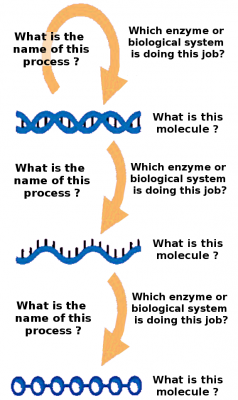
\includegraphics[scale=0.8]{centraldogmaex}
\end{figure}

Definitions
\begin{itemize}
\item tRNA
\item DNA Polymerase
\item nucleus
\item DNA
\item Protein
\item Transcription
\item Replication
\item codon
\item RNA polymerase
\item Ribosome
\item mRNA
\item Translation
\end{itemize}

\end{Exercise}

\begin{Answer} [
  ref={ex41},
  number={1}
 ]

\Question 
\begin{figure}[H]
\centering
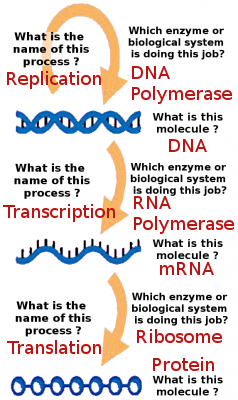
\includegraphics[scale=0.8]{centraldogmarx}
\end{figure}

\end{Answer}

\begin{Exercise} [
  label={ex42},
  origin={G. Valle}
 ]

\Question What is the expected percentage (approximate to the nearest integer)
of the genome covered by at least 3 reads?

\end{Exercise}

\begin{Answer} [
  ref={ex42},
  number={1}
 ]

\Question Our average coverage is 2. This is the variable ``r'' in the above
formula, or the term ``mean'' in the poisson function of an excel spreadsheet.
With the formula of the Poisson distribution we can calculate the expected
fraction of bases covered 0, 1 , 2, 3, etc times. To get the fraction of bases
covered at least 3 times we must consider that those covered 0, 1 and 2 times
should not be considered as "good", therefore from 100\% we should remove the
expected fraction of bases covered 0, 1 , and 2 times:
expected fraction of bases covered 0 times = 14\%
expected fraction of bases covered 1 time = 27\%
expected fraction of bases covered 2 times = 27\%
Final result: 100-14-27-27= 32\%
\end{Answer}


\begin{Exercise} [
  label={ex43},
  origin={G. Valle}
 ]

We have discussed about the experiment shown in this figure, demonstrating in
vitro evolution of RNA:

\begin{figure}[H]
\centering
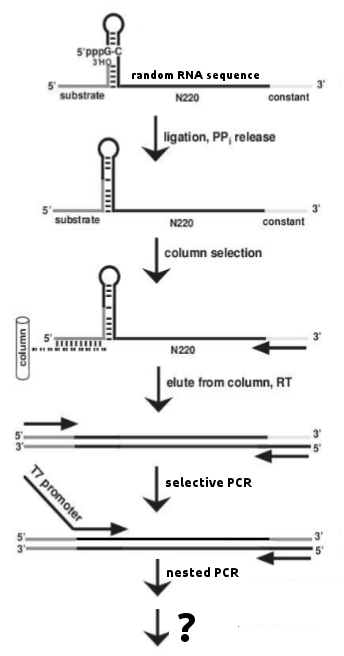
\includegraphics[scale=0.5]{rnainvitro}
\end{figure}

\Question Choose one or more answers:
\begin{enumerate}
\item It was for the selection of an RNA able to bind ATP
\item It was for the selection of an RNA able to catalyse a reaction of RNA
ligation
\item It was for the selection of an RNA able to covalently bind an amino acid
\item After the ``nested PCR'' reaction,  the PCR product can be immediately
used to repeat the cycle
\item After the ``nested PCR'' reaction,  the PCR product is used as a template
for transcription before repeating the cycle 
\end{enumerate}

\end{Exercise}

\begin{Answer} [
  ref={ex43},
  number={1}
 ]

\Question It was for the selection of an RNA able to catalyse a reaction of RNA
ligation, After the ``nested PCR'' reaction, the PCR product is used as a
template for transcription before repeating the cycle

\end{Answer}

\begin{Exercise} [
  label={ex44},
  origin={G. Valle}
 ]

\Question Match figures and lists with definitions\\
(a)
\begin{figure}[H]
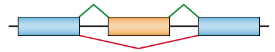
\includegraphics[scale=0.5]{splicinga}
\end{figure}
(b)
\begin{figure}[H]
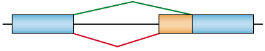
\includegraphics[scale=0.5]{splicingb}
\end{figure}
(c)
\begin{figure}[H]
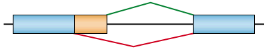
\includegraphics[scale=0.5]{splicingc}
\end{figure}
(d)
\begin{figure}[H]
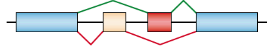
\includegraphics[scale=0.5]{splicingd}
\end{figure}
(e)
\begin{figure}[H]
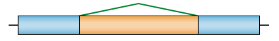
\includegraphics[scale=0.5]{splicinge}
\end{figure}
(f) ESE, ISE, ESS, ISS
(g) SR proteins, HnRNPs

Definitions
\begin{enumerate}
\item Mutually exclusive
\item Cis-acting elements
\item Trans-acting elements
\item Intron inversion
\item Exon skipping/inclusion
\item Alternative 3' splice sites
\item Intron retention
\item Alternative 5' splice sites
\end{enumerate}

\end{Exercise}

\begin{Answer} [
  ref={ex44},
  number={1}
 ]

\Question 
\begin{itemize}
\item fig. a - Exon skipping/inclusion
\item fig. b - Alternative 3' splice sites
\item fig. c - Alternative 5' splice sites
\item fig. d - Mutually exclusive
\item fig. e - Intron retention
\item f. ESE, ISE, ESS, ISS - Cis-acting elements
\item g. SR proteins, HnRNPs - Trans-acting elements
\end{itemize}
\end{Answer}